% Options for packages loaded elsewhere
% Options for packages loaded elsewhere
\PassOptionsToPackage{unicode}{hyperref}
\PassOptionsToPackage{hyphens}{url}
\PassOptionsToPackage{dvipsnames,svgnames,x11names}{xcolor}
%
\documentclass[
  number,
  review,
  3p]{elsarticle}
\usepackage{xcolor}
\usepackage{amsmath,amssymb}
\setcounter{secnumdepth}{5}
\usepackage{iftex}
\ifPDFTeX
  \usepackage[T1]{fontenc}
  \usepackage[utf8]{inputenc}
  \usepackage{textcomp} % provide euro and other symbols
\else % if luatex or xetex
  \usepackage{unicode-math} % this also loads fontspec
  \defaultfontfeatures{Scale=MatchLowercase}
  \defaultfontfeatures[\rmfamily]{Ligatures=TeX,Scale=1}
\fi
\usepackage{lmodern}
\ifPDFTeX\else
  % xetex/luatex font selection
\fi
% Use upquote if available, for straight quotes in verbatim environments
\IfFileExists{upquote.sty}{\usepackage{upquote}}{}
\IfFileExists{microtype.sty}{% use microtype if available
  \usepackage[]{microtype}
  \UseMicrotypeSet[protrusion]{basicmath} % disable protrusion for tt fonts
}{}
\makeatletter
\@ifundefined{KOMAClassName}{% if non-KOMA class
  \IfFileExists{parskip.sty}{%
    \usepackage{parskip}
  }{% else
    \setlength{\parindent}{0pt}
    \setlength{\parskip}{6pt plus 2pt minus 1pt}}
}{% if KOMA class
  \KOMAoptions{parskip=half}}
\makeatother
% Make \paragraph and \subparagraph free-standing
\makeatletter
\ifx\paragraph\undefined\else
  \let\oldparagraph\paragraph
  \renewcommand{\paragraph}{
    \@ifstar
      \xxxParagraphStar
      \xxxParagraphNoStar
  }
  \newcommand{\xxxParagraphStar}[1]{\oldparagraph*{#1}\mbox{}}
  \newcommand{\xxxParagraphNoStar}[1]{\oldparagraph{#1}\mbox{}}
\fi
\ifx\subparagraph\undefined\else
  \let\oldsubparagraph\subparagraph
  \renewcommand{\subparagraph}{
    \@ifstar
      \xxxSubParagraphStar
      \xxxSubParagraphNoStar
  }
  \newcommand{\xxxSubParagraphStar}[1]{\oldsubparagraph*{#1}\mbox{}}
  \newcommand{\xxxSubParagraphNoStar}[1]{\oldsubparagraph{#1}\mbox{}}
\fi
\makeatother


\usepackage{longtable,booktabs,array}
\usepackage{calc} % for calculating minipage widths
% Correct order of tables after \paragraph or \subparagraph
\usepackage{etoolbox}
\makeatletter
\patchcmd\longtable{\par}{\if@noskipsec\mbox{}\fi\par}{}{}
\makeatother
% Allow footnotes in longtable head/foot
\IfFileExists{footnotehyper.sty}{\usepackage{footnotehyper}}{\usepackage{footnote}}
\makesavenoteenv{longtable}
\usepackage{graphicx}
\makeatletter
\newsavebox\pandoc@box
\newcommand*\pandocbounded[1]{% scales image to fit in text height/width
  \sbox\pandoc@box{#1}%
  \Gscale@div\@tempa{\textheight}{\dimexpr\ht\pandoc@box+\dp\pandoc@box\relax}%
  \Gscale@div\@tempb{\linewidth}{\wd\pandoc@box}%
  \ifdim\@tempb\p@<\@tempa\p@\let\@tempa\@tempb\fi% select the smaller of both
  \ifdim\@tempa\p@<\p@\scalebox{\@tempa}{\usebox\pandoc@box}%
  \else\usebox{\pandoc@box}%
  \fi%
}
% Set default figure placement to htbp
\def\fps@figure{htbp}
\makeatother





\setlength{\emergencystretch}{3em} % prevent overfull lines

\providecommand{\tightlist}{%
  \setlength{\itemsep}{0pt}\setlength{\parskip}{0pt}}



 
\usepackage[]{natbib}
\bibliographystyle{elsarticle-harv}


\setcitestyle{authoryear,open={(},close={)}}
\makeatletter
\@ifpackageloaded{caption}{}{\usepackage{caption}}
\AtBeginDocument{%
\ifdefined\contentsname
  \renewcommand*\contentsname{Table of contents}
\else
  \newcommand\contentsname{Table of contents}
\fi
\ifdefined\listfigurename
  \renewcommand*\listfigurename{List of Figures}
\else
  \newcommand\listfigurename{List of Figures}
\fi
\ifdefined\listtablename
  \renewcommand*\listtablename{List of Tables}
\else
  \newcommand\listtablename{List of Tables}
\fi
\ifdefined\figurename
  \renewcommand*\figurename{Figure}
\else
  \newcommand\figurename{Figure}
\fi
\ifdefined\tablename
  \renewcommand*\tablename{Table}
\else
  \newcommand\tablename{Table}
\fi
}
\@ifpackageloaded{float}{}{\usepackage{float}}
\floatstyle{ruled}
\@ifundefined{c@chapter}{\newfloat{codelisting}{h}{lop}}{\newfloat{codelisting}{h}{lop}[chapter]}
\floatname{codelisting}{Listing}
\newcommand*\listoflistings{\listof{codelisting}{List of Listings}}
\makeatother
\makeatletter
\makeatother
\makeatletter
\@ifpackageloaded{caption}{}{\usepackage{caption}}
\@ifpackageloaded{subcaption}{}{\usepackage{subcaption}}
\makeatother
\journal{elsarticle}
\usepackage{bookmark}
\IfFileExists{xurl.sty}{\usepackage{xurl}}{} % add URL line breaks if available
\urlstyle{same}
\hypersetup{
  pdftitle={Predicting Auto Insurance Risk Using Gradient Boosting},
  pdfauthor={AJ Strauman-Scott},
  pdfkeywords={Gradient Boosting, XGBoost, SHAP
explainability, hyperparameter optimization, auto insurance
risk, American Community Survey (ACS), NYC Open Data, predictive
modeling, socio-economic predictors, crash modeling},
  colorlinks=true,
  linkcolor={blue},
  filecolor={Maroon},
  citecolor={Blue},
  urlcolor={Blue},
  pdfcreator={LaTeX via pandoc}}


\setlength{\parindent}{6pt}
\begin{document}

\begin{frontmatter}
\title{Predicting Auto Insurance Risk Using Gradient
Boosting \\\large{Analyzing Socio-Economic Factors in Car Crashes for
New York City} }
\author[1]{AJ Strauman-Scott%
%
}
 \ead{true} 

\affiliation[1]{organization={City University Of New York
(CUNY), Department of Data Science},city={New York City},country={United
States of America},countrysep={,},postcodesep={}}

\cortext[cor1]{Corresponding author}

        
\begin{abstract}
This study explores the use of the gradient boosting model XGBoost to
predict auto insurance risk by integrating socio-economic variables from
publicly available data. By treating crash frequency as proxy for
insurance claims, the project aims to identify key neighborhood-level
factors influencing risk. The dataset, encompassing 13,518 census
tract-by-year observations from 2018 to 2023, captures demographic,
economic, housing, and commuting indicators alongside engineered
interaction variables. Optuna hyperparameter tuning and SHAP-based
explainability reveal that post-pandemic traffic dynamics, median gross
rent, percent of a population in the labor-force, and the interaction of
poverty with vehicle ownership are significant predictors of crash risk.
While the model achieves moderate predictive accuracy (\(R^2\) = 0.425),
its interpretability highlights socio-economic disparities that
influence urban traffic safety. The findings underscore the potential of
open data-driven models for portfolio-level risk assessment and urban
safety planning, while cautioning against direct use for individual
underwriting due to fairness and legal concerns.
\end{abstract}





\begin{keyword}
    Gradient Boosting \sep XGBoost \sep SHAP
explainability \sep hyperparameter optimization \sep auto insurance
risk \sep American Community Survey (ACS) \sep NYC Open
Data \sep predictive modeling \sep socio-economic predictors \sep 
    crash modeling
\end{keyword}
\end{frontmatter}
    

\section{Introduction}\label{sec-intro}

Accurate insurance risk modeling is critical for setting fair premiums,
mitigating losses, and ensuring financial stability within the insurance
industry \citep{henckaerts, clemente}. Predicting claim frequency
supports pricing and enables insurers to manage portfolio-level risk and
optimize resource allocation \citep{mohamed}.

New York City (NYC) presents a complex urban environment where traffic
risks are shaped by socio-economic factors, dense infrastructure, and
scaling dynamics typical of large metropolitan areas
\citep{cabrera, bettencourt}. The availability of open datasets---such
as NYC's Motor Vehicle Collision (MVC) data and socio-economic
indicators from the American Community Survey (ACS)---offers a unique
opportunity to develop proxy models for insurance claim risk. These data
sources provide detailed insights into crash frequency, commuting
behaviors, and neighborhood-level demographics
\citep{adeniyi, brubacher}.

Traditional actuarial methods, such as Generalized Linear Models (GLMs),
have long been the foundation of risk pricing and underwriting due to
their interpretability and regulatory acceptance \citep{henckaerts}.
However, GLMs are limited in their ability to capture non-linear
relationships and interactions among complex predictors like
socio-economic factors, urban infrastructure, and driving behavior
\citep{clemente}. These limitations are particularly pronounced in urban
contexts, where crash risk is shaped by heterogeneous population
dynamics and localized factors \citep{cabrera, brubacher}.

Recent studies and systematic reviews confirm that machine learning
methods, particularly ensemble models like Gradient Boosting Machines
(GBMs), outperform traditional GLMs for predicting both claim frequency
and severity \citep{clemente, mohamed, behboudi}. These models are
capable of handling mixed data types (categorical and continuous) and
capturing complex feature interactions that linear models often miss.

To address the interpretability challenge of ``black box'' ML models,
SHAP (SHapley Additive exPlanations) offers a principled framework for
feature attribution, allowing insurers and policymakers to understand
both global feature importance and instance-level predictions
\citep{lundberg, dong, ning}. This combination of high-performance
prediction and explainability provides a strong foundation for modern
risk modeling \citep{kim}.

Despite the growing body of work applying GBMs to insurance modeling,
few studies integrate publicly available crash data with socio-economic
indicators to model claim-related risks specifically for the automotive
insurance sector. Most research remains limited to proprietary
policyholder data \citep{henckaerts, mohamed}, while systematic reviews
highlight that few studies combine open crash data with socio-economic
indicators in insurance modeling \citep{ali, behboudi}.

This study aims to integrate ACS socio-economic features with NYC MVC
crash data to develop an explainable gradient boosting framework for
measuring social risk for automotive insurance and urban policy. The
ultimate goal is to identify key socio-economic, transportation, and
demographic predictors that drive claim frequency, and to determine how
much crash risk can be predicted solely by these factors using an
XGBoost model, without incorporating weather, road pattern or
individual-level driver data.

The remainder of this paper is organized as follows: Section 2 reviews
prior work on ML in insurance risk modeling, model explainability, and
literature gaps; Section 3 details the data sources, key metrics,
modeling approach, and SHAP-based explainability; Section 4 reports the
results including hyperparameter tuning results, model performance, and
feature importance; Section 5 discusses the findings in relation to
existing research and industry applications; and Section 6 concludes
with key contributions, limitations, and directions for future research.

\section{Related Work}\label{sec-lit-review}

\subsection{\texorpdfstring{\textbf{Machine Learning in Insurance Risk
Modeling}}{Machine Learning in Insurance Risk Modeling}}\label{machine-learning-in-insurance-risk-modeling}

The transition from traditional actuarial models such as Generalized
Linear Models (GLMs) to machine learning (ML) approaches has marked a
significant evolution in insurance risk modeling. GLMs have historically
served as the backbone for pricing and claim prediction due to their
interpretability and regulatory acceptance. However, they are limited by
their linearity and inability to naturally capture complex interactions
and nonlinear relationships among predictors, such as driver
demographics, vehicle characteristics, socio-economic factors, and
driving behavior. As \citet{clemente} note, while GLMs remain effective
for modeling claim severity with smaller and noisier datasets, they
often underperform compared to ensemble methods when modeling claim
frequency, where nonlinearities and heterogeneous risk patterns are
prevalent. Similarly, \citet{jonkheijm} demonstrated that tree-based
models, especially XGBoost, substantially improved predictive accuracy
over linear regression, particularly when incorporating both actuarial
features (e.g., policyholder age, vehicle value) and behavioral
indicators.

Recent studies have validated the predictive superiority of ML
methods---such as random forests, GBMs, and neural networks---over
traditional actuarial models. GBMs, such as XGBoost and LightGBM, have
emerged as particularly effective tools in auto insurance risk modeling
\citep{henckaerts}. Their iterative boosting framework enables them to
handle mixed data types (categorical and continuous) and capture
intricate patterns that GLMs and single decision trees may miss.
\citet{clemente} applied gradient boosting to both claim frequency and
severity modeling, demonstrating significant performance gains in
frequency prediction over Poisson-based GLMs. Similarly,
\citet{jonkheijm} employed XGBoost for forecasting individual claim
amounts, outperforming both regression trees and random forests.

\subsection{\texorpdfstring{\textbf{Use of Crash and Socio-Economic
Data}}{Use of Crash and Socio-Economic Data}}\label{use-of-crash-and-socio-economic-data}

Crash data has been widely recognized as a reliable proxy for insurance
claim frequency, given the direct link between the occurrence of traffic
accidents and subsequent claims filed by policyholders. Studies
utilizing police crash reports, telematics, and open transportation
datasets consistently demonstrate strong correlations between crash
frequency and insurance risk metrics \citep{takale}.

The integration of socio-economic features---including income levels,
commuting patterns, vehicle ownership rates, and population
density---has been shown to enhance the explanatory power of crash and
claim prediction models. For example, \citet{adeniyi} utilized a decade
of NYC crash data (2013--2023) to identify key predictors of accident
severity---such as unsafe speed, alcohol involvement, and adverse
weather---which align closely with the variables insurers use to model
claim likelihood. Similarly, \citet{dong} applied boosting-based
ensemble models to traffic injury severity prediction, finding that
vehicle type, collision mode, and environmental conditions strongly
influenced both injury outcomes and, by extension, potential claim
costs. \citet{brubacher} conducted a geospatial analysis of 10 years of
crashes in British Columbia and found that regions with lower income and
higher socio-economic deprivation exhibited higher rates of pedestrian
crashes, severe injuries, and fatalities, reflecting disparities in road
safety linked to infrastructure quality and enforcement intensity.
\citet{cabrera} expanded on this by identifying superlinear scaling of
road accidents in urban areas, where higher population densities led to
disproportionate increases in crash frequency, especially for minor
collisions. These findings are directly relevant for insurers, as they
imply that socio-economic and urban structural factors---such as
commuting patterns or access to public transit---can serve as proxies
for underlying risk exposure.

Urban-focused studies have further illuminated the unique risk dynamics
in metropolitan environments like New York City, Chicago, and London,
where complex traffic patterns, dense road networks, and high pedestrian
activity elevate accident risk. \citet{adeniyi} analyzed NYC crash data
to show how the COVID-19 pandemic altered accident patterns, with fewer
total crashes but an increase in injury severity due to higher vehicle
speeds on less congested roads. \citet{feng}, studying UK traffic data,
emphasized the value of big data platforms and spatial clustering
techniques (e.g., accident hotspot detection) to identify urban risk
zones, a concept that parallels insurer efforts to assess region-based
risk for underwriting.

\subsection{\texorpdfstring{\textbf{Explainability in GBM
Models}}{Explainability in GBM Models}}\label{explainability-in-gbm-models}

In high-stakes fields such as insurance pricing, underwriting, and
claims management, the interpretability of ML models is not only a
technical preference but also a regulatory and business requirement.
Insurers must be able to justify rating factors and risk scores to
regulators, policyholders, and internal stakeholders. Traditional
actuarial models like GLMs are naturally interpretable due to their
linear structure and explicit coefficient estimates. However, modern ML
models---such as gradient boosting or neural networks---are often
criticized as ``black boxes,'' complicating the explanation of
predictions that influence financial decisions or customer premiums.
Regulatory frameworks, including the EU's General Data Protection
Regulation (GDPR) and U.S. state-level insurance guidelines,
increasingly require transparency in algorithmic decision-making,
further amplifying the need for explainable AI (shortened to XAI).
\citet{henckaerts} further underscore this, showing that variable
importance plots and partial dependence plots (PDPs) can yield
actionable insights into driver and policyholder risk factors, blending
predictive power with interpretability.

Among XAI methods, SHAP (SHapley Additive exPlanations) has become the
state-of-the-art framework for interpreting complex ML models. Developed
by \citet{lundberg}, SHAP is grounded in cooperative game theory,
assigning each feature a Shapley value that quantifies its contribution
to individual predictions. Unlike traditional feature importance
metrics---such as Gini importance in random forests or split gain in
XGBoost---SHAP accounts for both main effects and feature interactions,
offering a consistent and additive explanation of how variables drive
model outputs.

In the insurance domain, SHAP has been widely applied to interpret
models for claims prediction, fraud detection, and risk scoring.
\citet{dong} used SHAP in conjunction with boosting-based models
(LightGBM and CatBoost) to analyze the contribution of driver age,
vehicle type, and collision type to injury severity predictions,
providing insights that aligned with domain expertise. Similarly,
\citet{ning} demonstrated how Shapley Variable Importance Cloud
(ShapleyVIC) builds on SHAP principles to assess variable significance
with uncertainty intervals, enabling fairer and more transparent risk
predictions.

\subsection{\texorpdfstring{\textbf{Gaps in the
Literature}}{Gaps in the Literature}}\label{gaps-in-the-literature}

While ML methods---particularly ensemble models like gradient
boosting---have gained traction in insurance risk modeling, there is a
notable absence of studies that combine socio-economic and crash data
for claim risk prediction. Most existing research focuses on proprietary
insurance datasets containing policyholder and vehicle information
\citep{clemente, henckaerts, jonkheijm}. This gap limits the development
of robust, regionally sensitive models that capture the real-world
interaction between crash frequency and socio-economic indicators.

\section{Materials and Methods}\label{sec-methods}

\subsection{\texorpdfstring{\textbf{Data
Sources}}{Data Sources}}\label{data-sources}

The data sources and preprocessing steps are designed to replicate key
factors used in actuarial risk models while incorporating broader
socio-economic and regional variables.

\subsubsection{\texorpdfstring{\textbf{Crash Data (Claim
Proxies)}}{Crash Data (Claim Proxies)}}\label{crash-data-claim-proxies}

Crash data is obtained from the NYC Motor Vehicle Collisions (MVC) Open
Data Portal, covering the years 2018--2023. These variables are
well-documented predictors of both accident severity and insurance
claims \citep{adeniyi, dong}.

Crash frequency was aggregated at the 2020 census tract level and
normalized by tract-level population to compute crashes per 1,000
resident. This metric will replace claim frequency \citep{brubacher}.

\subsubsection{\texorpdfstring{\textbf{Socio-Economic Data (ACS
Features)}}{Socio-Economic Data (ACS Features)}}\label{socio-economic-data-acs-features}

Socio-economic variables are drawn from the ACS 5-year estimates
(2018--2023) at the 2020 census tract level. The variables include
demographic composition , age distribution, and income indicators.
Additional features include median gross rent, housing tenure,
educational attainment, employment metrics, and transportation factors.
The full table of ACS derived variables in available in
Section~\ref{sec-appA}.

\subsection{\texorpdfstring{\textbf{Key
Metrics}}{Key Metrics}}\label{key-metrics}

The primary risk metric, \texttt{crash\_rate\_per\_1000}, measures the
number of crashes per 1,000 residents in each census tract by year. This
population-adjusted rate follows the methodology of studies that
normalize crash counts by population to ensure fair comparisons of
relative risk across areas with varying exposure levels
\citep{brubacher, cabrera}.

This response variable is modeled alongside the transformed and selected
socio-economic and transportation variables detailed in
Section~\ref{sec-appB}. Together, these variables allow the model to
capture both the exposure risk (frequency) and potential cost severity
of accidents, aligning with the frameworks used in both insurance
\citep{clemente, henckaerts} and traffic safety research \citep{dong}.

\subsubsection{\texorpdfstring{\textbf{Preprocessing}}{Preprocessing}}\label{preprocessing}

Crash records from the NYC Open Data MVC dataset are spatially joined to
2020 Census Tracts using official census tract shapefiles. Annual
summaries of total crashes, injuries, and fatalities are then aggregated
by tract and normalized by tract-level population to compute annual
per-capita crash rates for each census tract in NYC for each year.

The ACS socio-economic data are harmonized to 2020 tract boundaries (via
crosswalks for 2018--2019), binned into interpretable categories, and
converted to percentages of total population where applicable.
Interaction features-poverty rate and vehicle ownership, as well as
unemployment rate and vehicle ownership-were engineered to capture
compound effects on risk exposure.

After examination, a subset of highly correlated variables were removed.
Measures of poverty level and population above the poverty line, as well
as employment and unemployment percentages, were closely tied to broader
income and labor force indicators already included in the model,
creating redundancy without improving predictive power. Similarly,
metrics describing commuting alone by car and the distribution of
vehicle ownership were binned to prevent issues from being strongly
interrelated. The precentage of female share of the population was
excluded because of its near-perfect correlation with the male share of
the population. The same was true for the share of high-income
households, which closely overlapped with median income levels.

No categorical encoding besides \texttt{year} or feature standardization
was performed, as all ACS predictors are expressed as continuous
percentages or numeric values, and gradient boosting models (XGBoost)
handle raw scales effectively \citep{henckaerts}. However, the response
variable - number of crashes per 1,000 people - was log-transformed to
stabilize variance and reduce the impact of extreme values.

\subsection{\texorpdfstring{\textbf{Modeling
Approach}}{Modeling Approach}}\label{modeling-approach}

XGBoost \citep{xgboost} is chosen for its strong track record in
insurance risk modeling and interpretability when combined with SHAP
\citep{dong}. This model selection aligns with studies comparing
boosting frameworks for both frequency-severity modeling
\citep{henckaerts} and urban crash prediction \citep{adeniyi}.

Model performance was optimized with hypermater tuning using the
automated Bayesian optimization framework Optuna \citep{optuna}. This
approach is supported by prior research showing that systematic
hyperparameter optimization significantly improves boosting model
accuracy \citep{liu}.

Each configuration of Optuna tuning was evaluated using spatial
cross-validation at the borough level on the training data to balance
bias and variance, ensuring that the model captured meaningful patterns
without overfitting or overgeneralizing across geography.

\section{Results}\label{results}

\subsection{\texorpdfstring{\textbf{Descriptive
Statistics}}{Descriptive Statistics}}\label{descriptive-statistics}

The dataset comprises 13,518 census tract--year observations from 2018
to 2023. Population counts vary widely across tracts, with a median of
approximately 42,979 residents and extremes ranging from fewer than 100
to over 220,000.

\begin{figure}[H]

\centering{

\pandocbounded{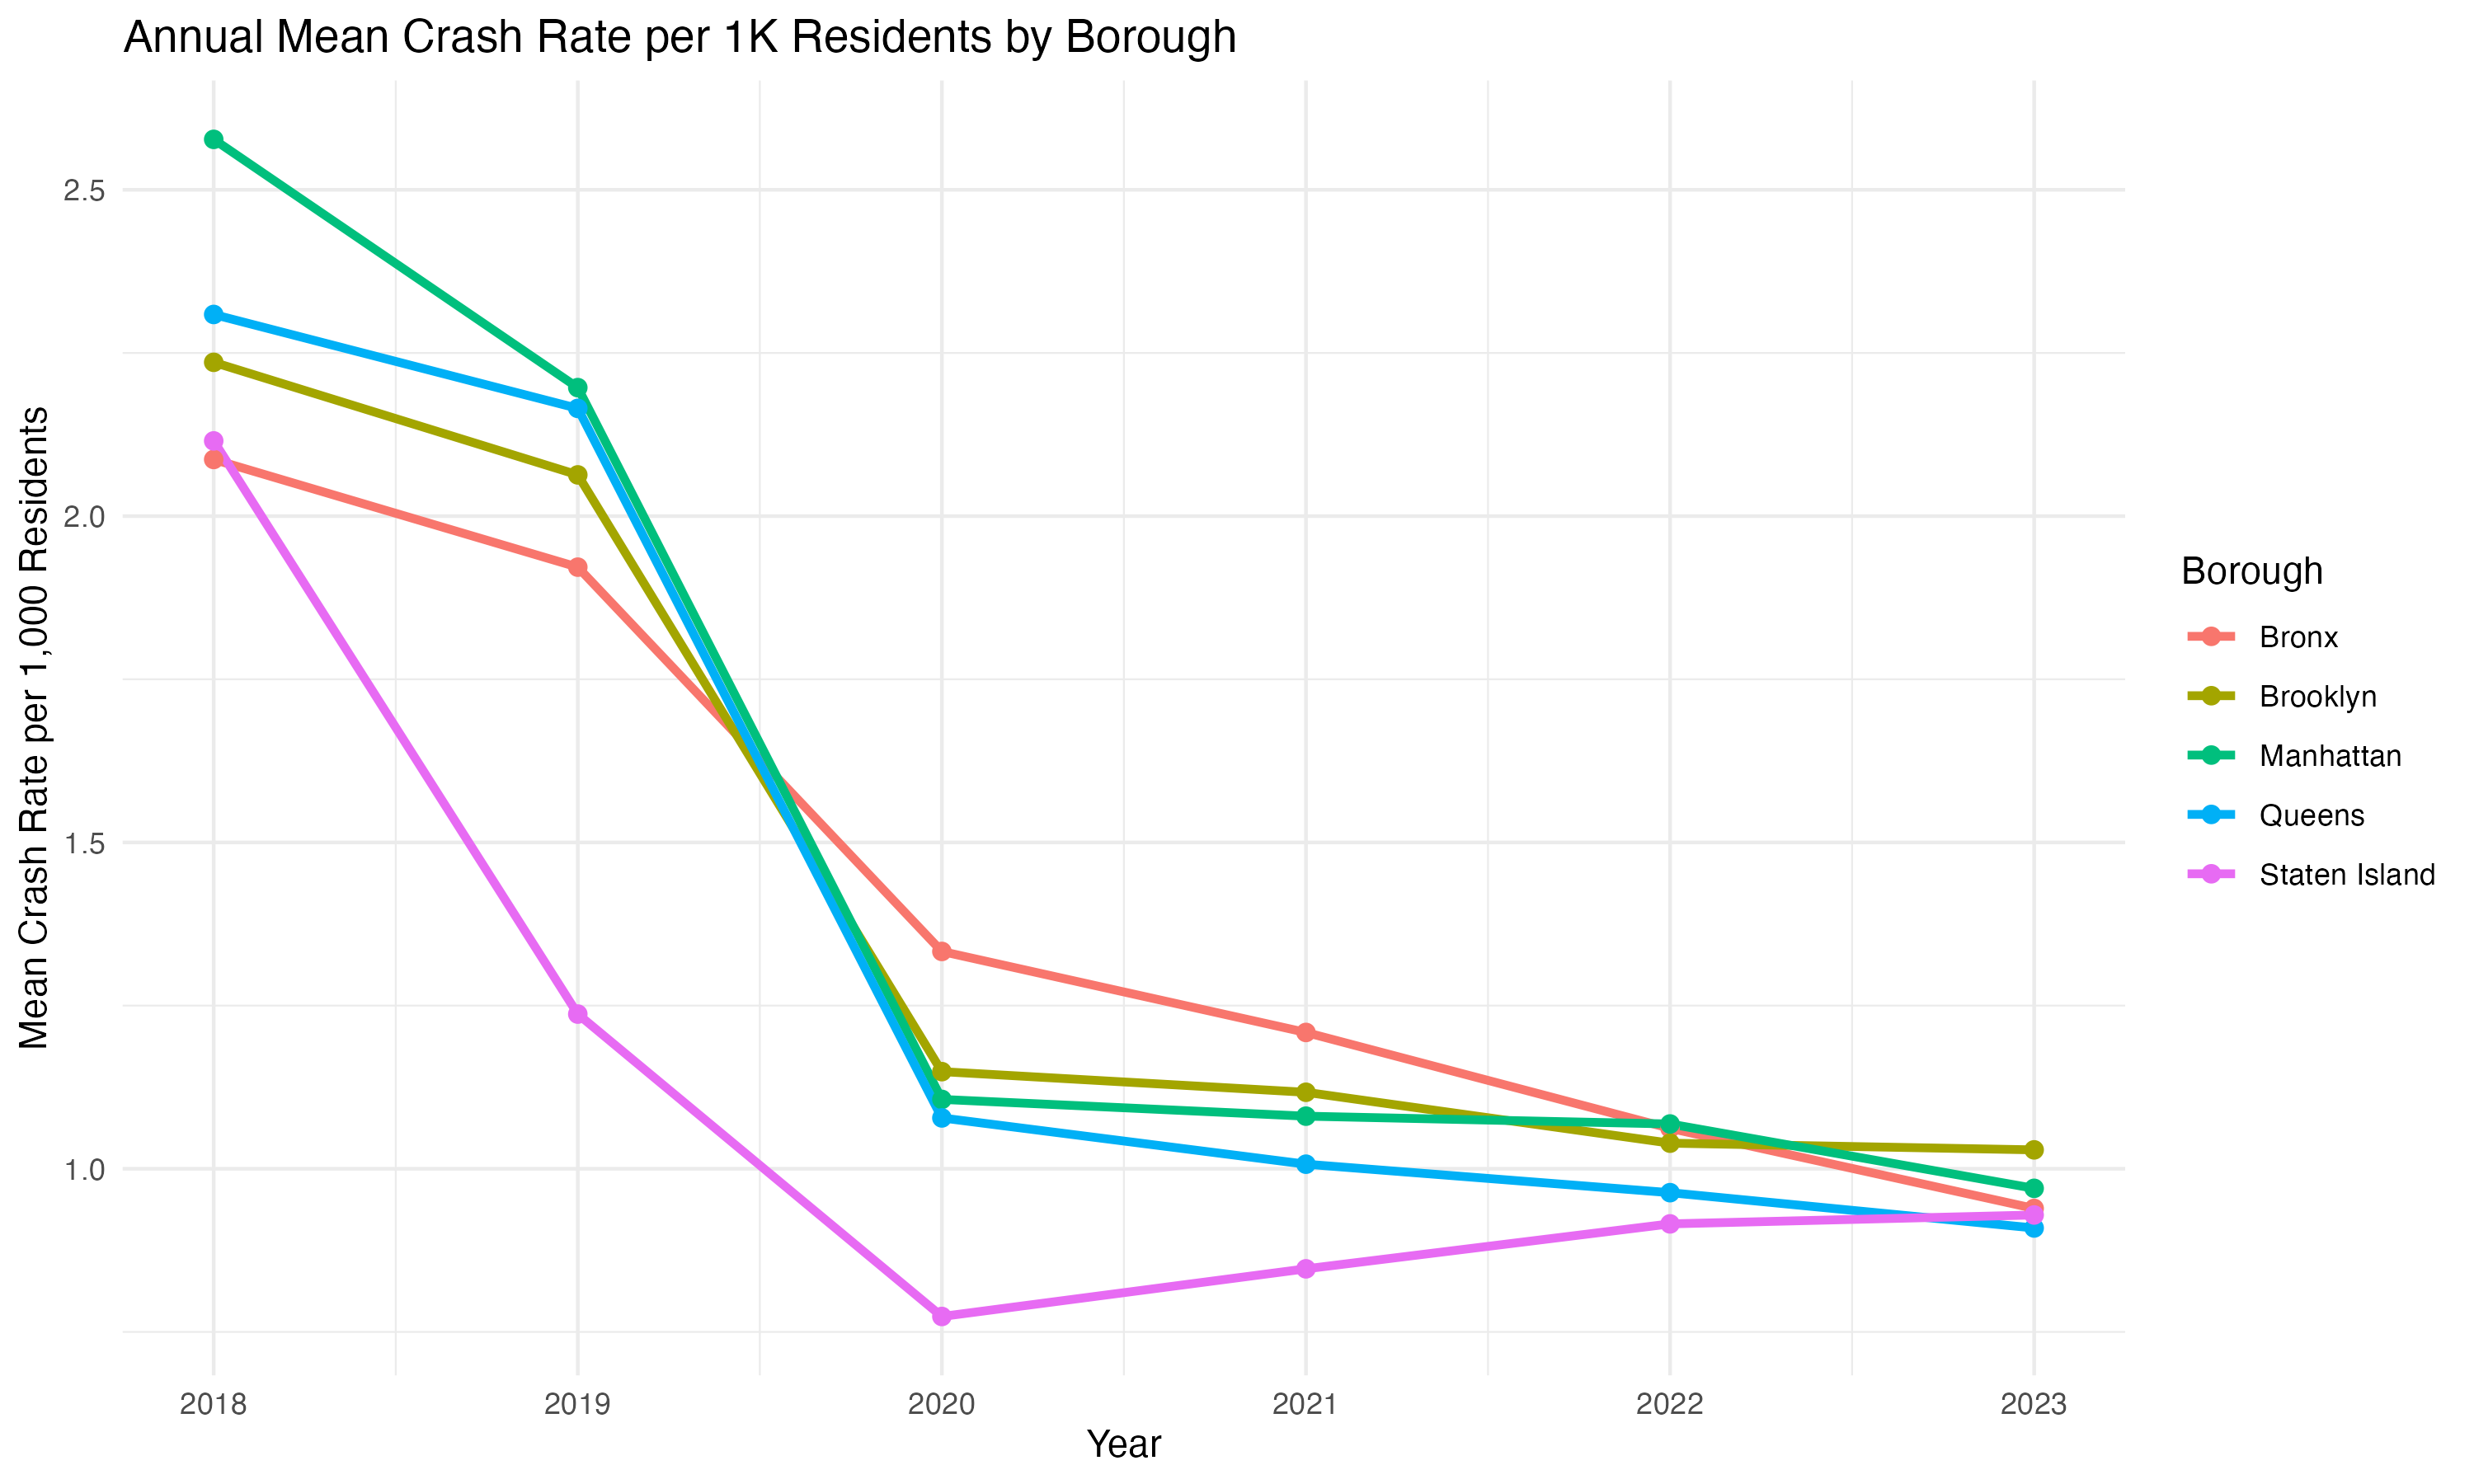
\includegraphics[keepaspectratio]{plots/crash_rate_by_borough_plot.png}}

}

\caption{\label{fig-crashes}Crash Rate by Borough, by Year}

\end{figure}%

In Figure~\ref{fig-crashes}, crash rate by borough shows a clear
downward trend in crash rates across all boroughs over time, with a
sharp reduction during the COVID-19 pandemic period (2020) and gradual
stabilization afterward. Bronx and Queens consistently show higher crash
rates per 1,000 residents compared to Staten Island and Manhattan.

\begin{figure}[H]

\centering{

\pandocbounded{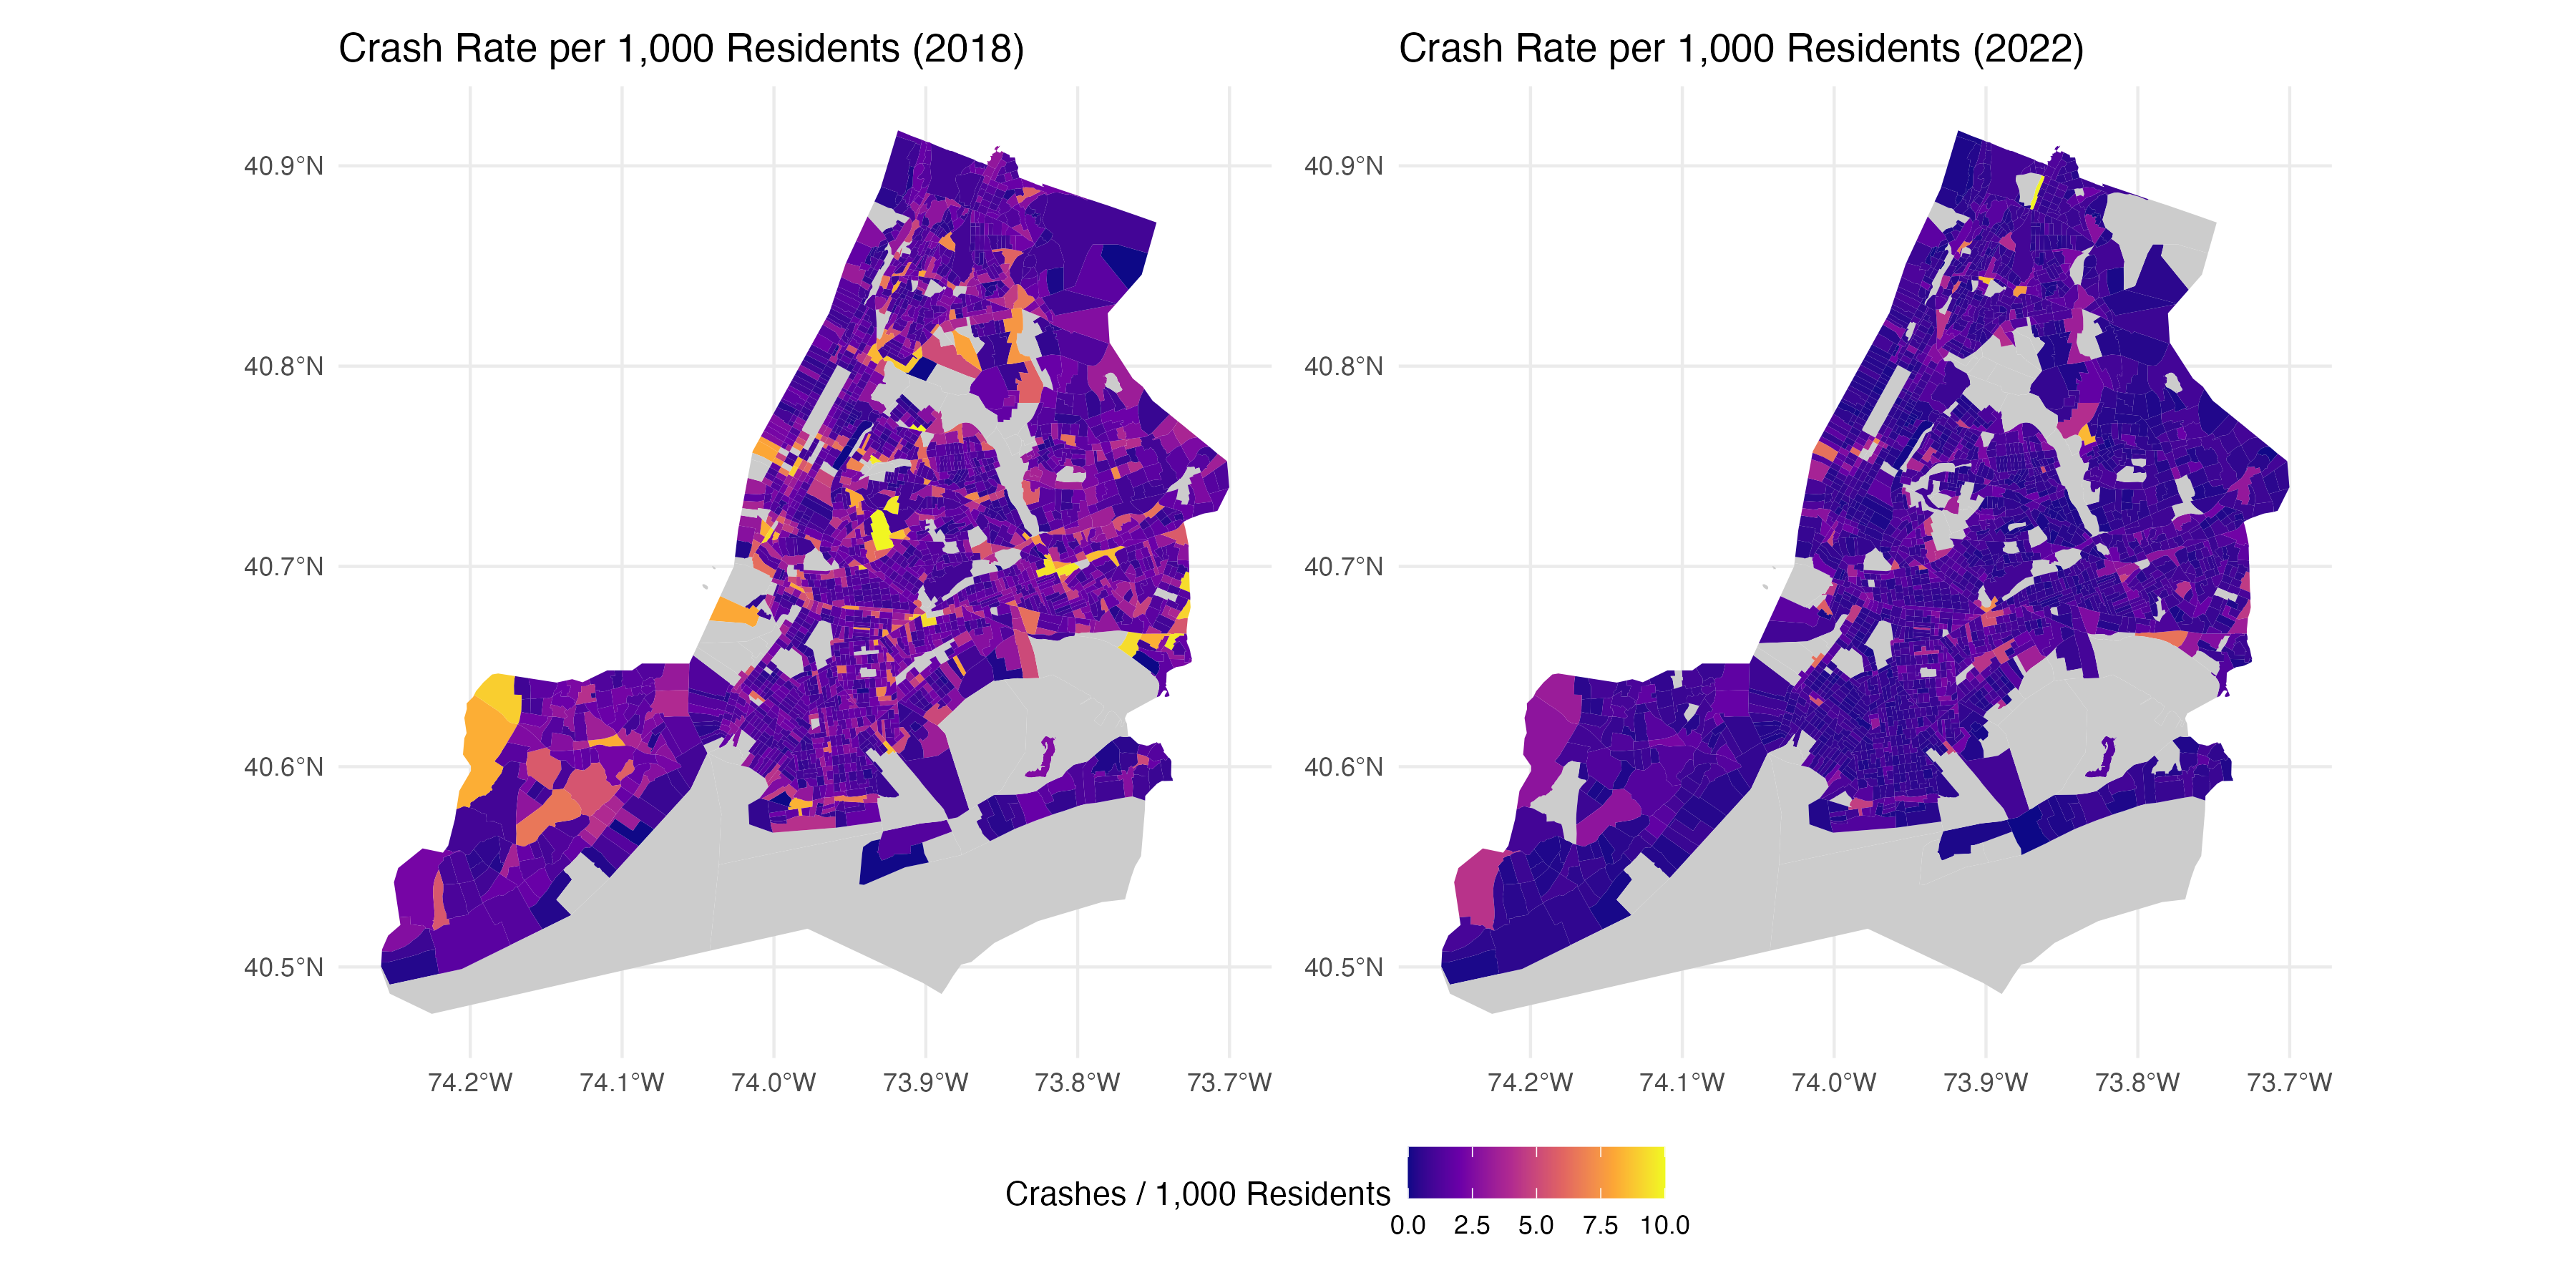
\includegraphics[keepaspectratio]{plots/2018_2022_comparison.png}}

}

\caption{\label{fig-heatmap}Crash Rate in 2018 vs 2022}

\end{figure}%

The geospatial heatmaps in Figure~\ref{fig-heatmap} illustrate how crash
rates are spatially clustered within the city. In 2018, high crash rates
were concentrated in central Brooklyn, the South Bronx, and sections of
northern Manhattan, while in 2022, these hotspots persisted but appeared
less intense overall, consistent with the downward temporal trend across
both total and commuting population post-Covid-19 pandemic. Applying the
same color scale across both maps, it is evident that most census tracts
saw a reduction in crash intensity, although isolated high-risk
corridors remain.

\subsection{\texorpdfstring{\textbf{Hyperperameter
Tuning}}{Hyperperameter Tuning}}\label{hyperperameter-tuning}

Optuna hyperparameter tuning \citep{optuna} enhanced the predictive
accuracy and generalization capability of the XGBoost model. The final
configuration represents a balance between model complexity and
overfitting risk, as determined by performance on the training and
validation subsets.

\begin{longtable}[]{@{}lll@{}}
\caption{Optimal Parameters as per Optuna}\tabularnewline
\toprule\noalign{}
Action & Parameter & Value \\
\midrule\noalign{}
\endfirsthead
\toprule\noalign{}
Action & Parameter & Value \\
\midrule\noalign{}
\endhead
\bottomrule\noalign{}
\endlastfoot
Learning Rate & \texttt{eta} & 0.2586295 \\
Tree Depth & \texttt{max\_depth} & 12 \\
Row Sampling & \texttt{subsample} & 0.9921435 \\
Feature Sampling & \texttt{colsample\_bytree} & 0.5823858 \\
Minimum Child Weight & \texttt{min\_child\_weight} & 4 \\
Minimum Loss Reduction & \texttt{gamma} & 0.08316905 \\
L2 Regularization & \texttt{lambda} & 4.260907 \\
L1 Regularization & \texttt{alpha} & 0.2049112 \\
\end{longtable}

The tree depth of 12 allows the model to make much deeper splits,
capturing highly granular interactions between socio-economic and
crash-related variables. While deep trees can increase the risk of
overfitting, this is balanced by the other constraints in the model. The
minimum child weight places a threshold on the minimum sum of instance
weights required to create a split. This prevents the model from
building branches that explain only a small subset of observations,
helping to maintain focus on broader patterns in the data.

The learning rate is moderate, enabling the model to update predictions
in steady increments without being overly aggressive. This value strikes
a balance between convergence speed and stability.

The row sampling rate (\texttt{subsample\ =\ 0.992}) indicates that
nearly all rows are used in each boosting iteration, which reduces
variance but increases the risk of memorizing noise in the data. In
contrast, the feature sampling rate
(\texttt{colsample\_bytree\ =\ 0.582}) introduces meaningful randomness
by selecting slightly more than half of the features for each tree.

Regularization parameters, \texttt{lambda} (L2) and \texttt{alpha} (L1),
apply moderate constraints to the feature weights, discouraging overly
complex or extreme splits without overly penalizing flexibility. The
minimum loss reduction (\texttt{gamma} = 0.083) is relatively low, which
allows the model to explore more potential splits during training. This
can enhance the model's ability to capture subtle relationships between
features.

\subsection{\texorpdfstring{\textbf{Model
Performance}}{Model Performance}}\label{model-performance}

The XGBoost model achieved robust predictive performance on the holdout
test set, with the following metrics:

\begin{longtable}[]{@{}ll@{}}
\caption{XGBOOST Model Evaluation Metrics}\tabularnewline
\toprule\noalign{}
Metric & Score \\
\midrule\noalign{}
\endfirsthead
\toprule\noalign{}
Metric & Score \\
\midrule\noalign{}
\endhead
\bottomrule\noalign{}
\endlastfoot
RMSE & 0.3396146 \\
MAE & 0.2422538 \\
\(R^2\) & 0.425285 \\
\end{longtable}

These metrics indicate solid predictive performance with tight error
bounds relative to the normalized crash rate values. An RMSE of 0.34
suggests that predictions deviate by approximately 0.34 crashes per
1,000 residents on average, which is a low margin of error given the
variability across census tracts. The MAE of 0.24 confirms that typical
prediction errors remain well below half a crash per 1,000 residents.

Most critically, the \(R^2\) value of 0.43 means the model explains
approximately 43\% of the variance in crash rates, a strong result for a
model built only on socio-economic and transportation predictors,
without direct behavioral or vehicle-level data.

\begin{figure}[H]

{\centering \pandocbounded{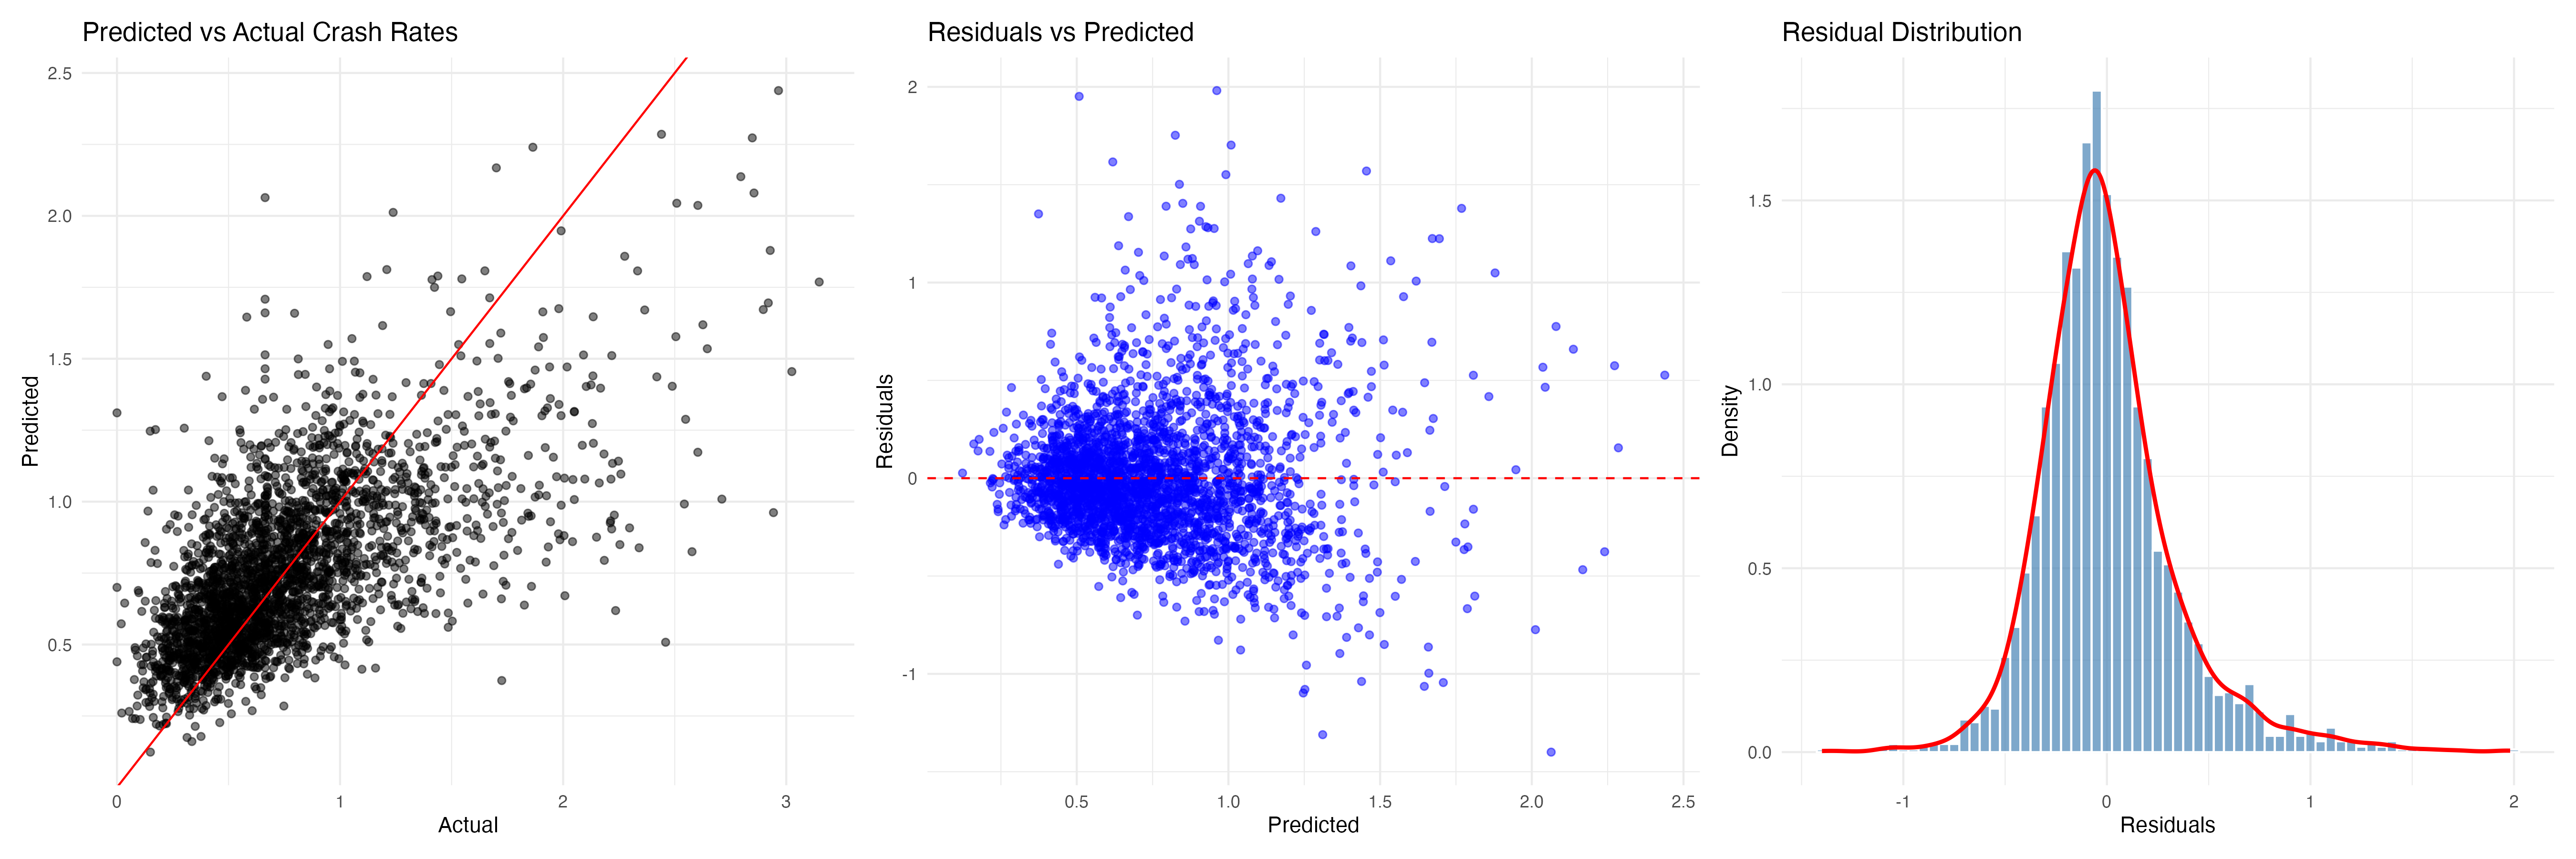
\includegraphics[keepaspectratio]{plots/residuals_diagnostic_grid.png}}

}

\caption{Residual Diagnostic Plots}

\end{figure}%

\subsubsection{\texorpdfstring{\textbf{Residuals}}{Residuals}}\label{residuals}

The predicted vs.~actual values plot shows that while the model
generally tracks the trend of observed crash rates, there is a clear
cone-shaped spread. This indicates that predictions tend to be
compressed toward the mean---with underestimation for high crash-rate
tracts and overestimation for low crash-rate tracts. This is a common
behavior for gradient boosting models trained on noisy data, where
extreme values are smoothed due to ensemble averaging.

The residuals vs.~predicted values plot also displays the same cone
shape. This pattern suggests variance increases at the extremes, meaning
the model is less confident and less accurate when predicting very high
or very low crash rates.

The residual distribution plot remains centered around zero with a sharp
peak, showing minimal systemic bias.

\subsection{\texorpdfstring{\textbf{Feature Importance
(SHAP)}}{Feature Importance (SHAP)}}\label{feature-importance-shap}

\begin{figure}[H]

{\centering \pandocbounded{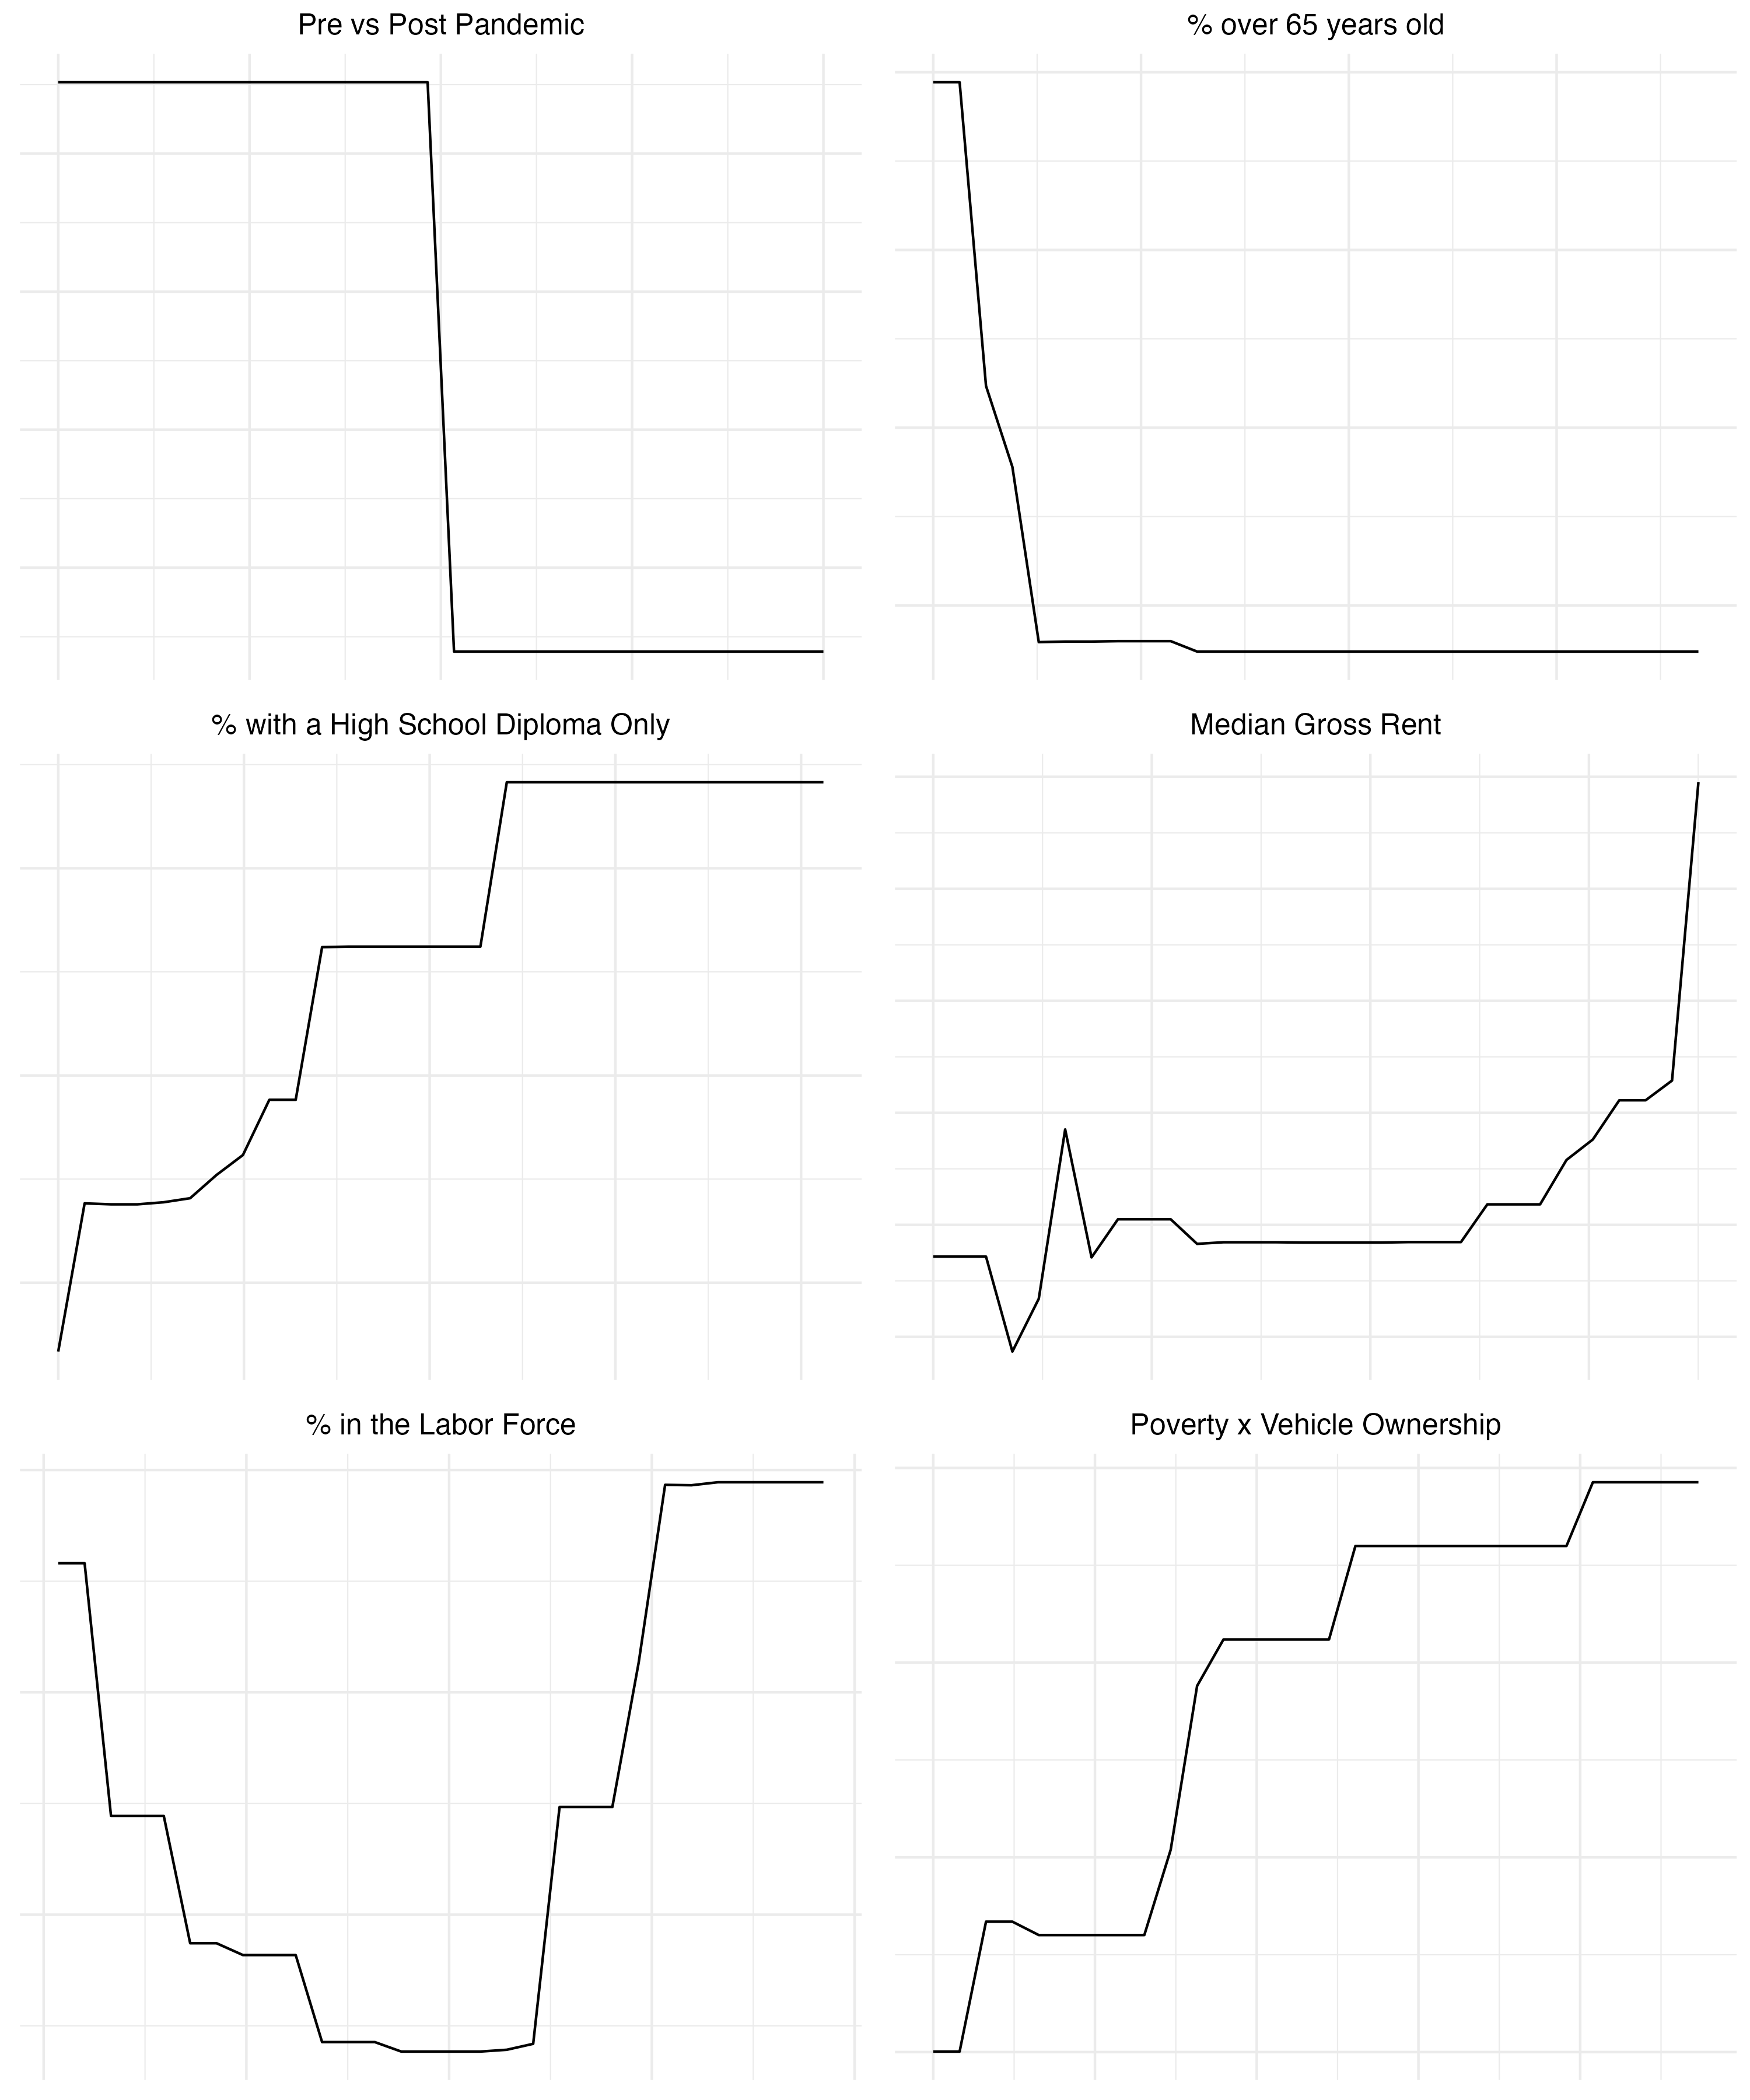
\includegraphics[keepaspectratio]{plots/pdp/pdp_grid.png}}

}

\caption{Global Feature Importance with SHAP}

\end{figure}%

The SHAP plot highlights the six most influential variables shaping
crash risk predictions in the XGBoost model. These features reveal
complex, non-linear relationships with crash rates:

\textbf{Post-Pandemic Indicator}

The pre vs.~post-COVID-19 variable shows a sharp drop in predicted crash
rates after the pandemic began, consistent with the reduction in traffic
volumes and changes in driving patterns observed citywide, also observed
by \citet{adeniyi}.

\textbf{Aging Population}

Crash risk declines as the proportion of residents aged 65 and older
increases up to roughly 2\%, likely due to reduced driving exposure
among elderly populations. Beyond this point, the trend stabilizes,
suggesting diminishing marginal effects.

\textbf{Graduate Degree Share}

The percentage of residents with graduate degrees exhibits a steady
downward relationship with crash risk. Higher educational attainment may
correlate with neighborhoods that have better infrastructure or lower
exposure to high-risk driving.

\textbf{Working Population}

The PDP for labor force participation indicates a non-linear trend.
Crash risk decreases slightly between 2\% and 5\% workforce
participation but increases sharply as participation exceeds 5\%,
reflecting higher commuter activity and vehicle miles traveled.

\textbf{Median Income}

Median income shows a non-monotonic relationship: risk is elevated in
very low-income areas, dips in middle-income neighborhoods, and then
rises again at high-income levels, possibly reflecting denser, high-cost
urban areas with complex traffic dynamics.

\textbf{Medium Commute Share} The percentage of residents with
medium-length commutes (15--30 minutes) is strongly associated with
higher crash risk once it exceeds approximately 3\%. This likely
reflects regions with heavier traffic flow and greater exposure to
collisions.

\section{Discussion}\label{discussion}

The XGBoost model achieved a notable performance with an \(R^2\) of
0.43, meaning it explains over 40\% of the variance in crash rates
across New York City census tracts. This is a strong result given the
absence of driver-level or vehicle-level data and the inherently
stochastic nature of traffic collisions. The low RMSE (0.34 crashes per
1,000 residents) and MAE (0.24) indicate that the model's predictions
are generally close to observed values, with small, consistent errors
across most census tracts.

From a social risk modeling perspective, the results highlight the
importance of broader socio-economic and transportation-related
conditions in shaping crash risk. The SHAP analysis reveals that the
post-pandemic indicator is the single strongest predictor, showing a
significant shift in traffic patterns starting in 2020. Reduced
congestion but increased vehicle speeds during and after the pandemic
contributed to changes in crash risk that conventional actuarial models
might fail to capture.

Key socio-economic variables also play prominent roles. Median income
exhibits a non-linear relationship with crash risk, with both very
low-income and high-income areas seeing higher risk---likely due to a
mix of infrastructure disparities and dense traffic flows. Labor force
participation and commute-related metrics, particularly the share of
medium-length commutes, are also strongly predictive, indicating that
commuter activity and roadway exposure remain fundamental drivers of
crash frequency. The negative association between graduate degree share
and crash risk may reflect safer traffic environments or reduced
reliance on driving in these neighborhoods.

These findings emphasize the interplay between economic conditions,
urban infrastructure, and mobility behaviors in shaping
neighborhood-level crash risks. High-income and low-income areas may
share common risk factors, such as higher vehicle ownership rates,
complex traffic flows, or limited access to safe pedestrian
infrastructure, albeit for different reasons. Similarly, commute-related
variables underscore the importance of traffic volume and duration as
core determinants of crash likelihood, suggesting that transportation
policies---such as investment in public transit or traffic-calming
measures---could meaningfully reduce risks

The cone-shaped residual patterns suggest that while the model performs
well across the midrange of crash rates, it tends to compress
predictions toward the mean---underestimating high-risk tracts and
overestimating low-risk ones. This limitation is typical for tree-based
ensembles trained on data with sparse extremes, but it indicates an
opportunity for refinement through log-transformed targets or quantile
regression techniques.

Although the model provides actionable insights into spatial risk
patterns, its direct use for individual insurance pricing is neither
appropriate nor ethical. Socio-economic and demographic factors, while
predictive, are not permissible as rating factors due to potential for
proxy discrimination. Instead, these findings are better suited for
identifying high-risk areas for targeted safety interventions, urban
planning efforts, or high-level portfolio analysis.

\section{Conclusions and Future Work}\label{conclusions-and-future-work}

This study demonstrates that gradient boosting models, when combined
with open crash and socio-economic data, can produce accurate and
interpretable models of neighborhood-level crash risk in New York City.
By identifying factors such as post-pandemic traffic changes, income
patterns, educational attainment, and commuting behaviors, the model
offers a rich, data-driven understanding of how socio-economic context
influences crash frequency.

However, the model's focus on aggregated census tract data and its
moderate \$R\^{}\$2 highlight the limits of what can be achieved without
driver-specific or telematics data. While it effectively captures
macro-level trends, it is not a replacement for traditional actuarial
models but rather a complementary tool for exploring spatial and
demographic risk factors.

Future research should focus on three fronts: (1) integrating behavioral
data, such as telematics, and weather patterns-among other possible
additions-to bridge the gap between macro-level socio-economic patterns
and micro-level driving behavior; (2) developing fairness-aware modeling
approaches to mitigate bias from socio-economic proxies; and (3)
exploring temporal extensions that incorporate evolving risk factors,
including post-pandemic traffic patterns and climate-related hazards.
These directions will help transition from descriptive social risk
modeling to actionable, ethically sound insurance applications.

\section{Appendix A: ACS Variables}\label{sec-appA}

\begin{longtable}[]{@{}
  >{\raggedright\arraybackslash}p{(\linewidth - 4\tabcolsep) * \real{0.0526}}
  >{\raggedright\arraybackslash}p{(\linewidth - 4\tabcolsep) * \real{0.1805}}
  >{\raggedright\arraybackslash}p{(\linewidth - 4\tabcolsep) * \real{0.7669}}@{}}
\caption{ACS tables and derived variables.}\tabularnewline
\toprule\noalign{}
\begin{minipage}[b]{\linewidth}\raggedright
ACS
\end{minipage} & \begin{minipage}[b]{\linewidth}\raggedright
Description
\end{minipage} & \begin{minipage}[b]{\linewidth}\raggedright
Derived.Variables
\end{minipage} \\
\midrule\noalign{}
\endfirsthead
\toprule\noalign{}
\begin{minipage}[b]{\linewidth}\raggedright
ACS
\end{minipage} & \begin{minipage}[b]{\linewidth}\raggedright
Description
\end{minipage} & \begin{minipage}[b]{\linewidth}\raggedright
Derived.Variables
\end{minipage} \\
\midrule\noalign{}
\endhead
\bottomrule\noalign{}
\endlastfoot
B01001 & Age and Sex & total\_population, male\_population,
female\_population, age\_under\_18, age\_18\_34, age\_35\_64,
age\_65\_plus \\
B08301 & Transportation to Work & drive\_alone, carpool,
public\_transit, walk, bike, work\_from\_home \\
B08303 & Travel Time to Work & commute\_short, commute\_medium,
commute\_long \\
B19001 & Household Income & income\_under\_25k, income\_25k\_75k,
income\_75k\_plus, median\_income \\
B25010 & Average Household Size & average\_household\_size \\
B25044 & Vehicles Available & no\_vehicle, one\_vehicle,
two\_plus\_vehicles \\
C24010 & Occupation & occupation variables (aggregated) \\
C24030 & Industry & industry variables (aggregated) \\
B15003 & Education & less\_than\_hs, hs\_diploma, some\_college,
associates\_degree, bachelors\_degree, graduate\_degree \\
B17001 & Poverty Status & below\_poverty, above\_poverty,
poverty\_rate \\
B02001 & Race & white\_population, black\_population,
asian\_population \\
B03002 & Hispanic or Latino & hispanic\_population \\
B16005 & Language Spoken at Home & foreign\_born \\
B23025 & Employment Status & in\_labor\_force, employed, unemployed,
not\_in\_labor\_force, unemployment\_rate \\
B25064 & Median Gross Rent & median\_gross\_rent \\
\end{longtable}

\section{Appendix B: Variables Modeled}\label{sec-appB}

\begin{longtable}[]{@{}
  >{\raggedright\arraybackslash}p{(\linewidth - 6\tabcolsep) * \real{0.1210}}
  >{\raggedright\arraybackslash}p{(\linewidth - 6\tabcolsep) * \real{0.2984}}
  >{\raggedright\arraybackslash}p{(\linewidth - 6\tabcolsep) * \real{0.4516}}
  >{\raggedright\arraybackslash}p{(\linewidth - 6\tabcolsep) * \real{0.1290}}@{}}
\caption{Key variables, descriptions, and transformations in the final
dataset.}\tabularnewline
\toprule\noalign{}
\begin{minipage}[b]{\linewidth}\raggedright
Variable
\end{minipage} & \begin{minipage}[b]{\linewidth}\raggedright
Description
\end{minipage} & \begin{minipage}[b]{\linewidth}\raggedright
Type
\end{minipage} & \begin{minipage}[b]{\linewidth}\raggedright
Transformation
\end{minipage} \\
\midrule\noalign{}
\endfirsthead
\toprule\noalign{}
\begin{minipage}[b]{\linewidth}\raggedright
Variable
\end{minipage} & \begin{minipage}[b]{\linewidth}\raggedright
Description
\end{minipage} & \begin{minipage}[b]{\linewidth}\raggedright
Type
\end{minipage} & \begin{minipage}[b]{\linewidth}\raggedright
Transformation
\end{minipage} \\
\midrule\noalign{}
\endhead
\bottomrule\noalign{}
\endlastfoot
Demographic & pct\_male\_population & Men & Percentage \\
Demographic & pct\_white\_population & Identifying as white &
Percentage \\
Demographic & pct\_black\_population & Identifying as black &
Percentage \\
Demographic & pct\_asian\_population & Identifying as Asian &
Percentage \\
Demographic & pct\_hispanic\_population & Identifying as Hispanic/Latino
& Percentage \\
Demographic & pct\_foreign\_born & Foreign-born & Percentage \\
Age & pct\_age\_under\_18 & Under 18 & Percentage \\
Age & pct\_age\_18\_34 & Aged 18-34 & Percentage \\
Age & pct\_age\_35\_64 & Aged 35-64 & Percentage \\
Age & pct\_age\_65\_plus & Aged 65 and above & Percentage \\
Income/Poverty & median\_income & Median household income
(inflation-adjusted) & Raw value (USD) \\
Income/Poverty & pct\_income\_under\_25k & Households earning less than
\$25,000 & Percentage \\
Income/Poverty & pct\_income\_25k\_75k & Households earning
\$25,000-\$75,000 & Percentage \\
Income/Poverty & pct\_below\_poverty & Below the poverty line &
Percentage \\
Housing & median\_gross\_rent & Median gross rent (USD) & Raw value
(USD) \\
Housing & pct\_owner\_occupied & Owner-occupied housing units &
Percentage \\
Housing & pct\_renter\_occupied & Renter-occupied housing units &
Percentage \\
Education & pct\_less\_than\_hs & Less than high school education &
Percentage \\
Education & pct\_hs\_diploma & High school diploma & Percentage \\
Education & pct\_some\_college & Some college education & Percentage \\
Education & pct\_associates\_degree & Associate's degree & Percentage \\
Education & pct\_bachelors\_degree & Bachelor's degree & Percentage \\
Education & pct\_graduate\_degree & Graduate or professional degree &
Percentage \\
Employment & pct\_in\_labor\_force & In the labor force & Percentage \\
Employment & unemployment\_rate & Unemployment rate & Percentage \\
Transport & pct\_commute\_short & Commute under 15 minutes &
Percentage \\
Transport & pct\_commute\_medium & Commute between 15-30 minutes &
Percentage \\
Transport & pct\_commute\_long & Commute longer than 30 minutes &
Percentage \\
Transport & pct\_carpool & By carpool & Percentage \\
Transport & pct\_public\_transit & By public transit & Percentage \\
Transport & pct\_walk & By walking & Percentage \\
Transport & pct\_bike & By biking & Percentage \\
Transport & pct\_work\_from\_home & Working from home & Percentage \\
Transport & pct\_vehicle & Owns a vehicle & Percentage \\
Engineered & post\_pandemic & Post-pandemic indicator (1 = 2020 and
later) & Binary \\
Engineered & poverty\_vehicle & & \\
\_interaction & Interaction term: poverty rate × vehicle ownership &
Interaction & \\
Engineered & unemployment\_vehicle & & \\
\_interaction & Interaction term: unemployment rate × vehicle ownership
& Interaction & \\
Year & year2018 & Year dummy: 2018 & Indicator \\
Year & year2019 & Year dummy: 2019 & Indicator \\
Year & year2020 & Year dummy: 2020 & Indicator \\
Year & year2021 & Year dummy: 2021 & Indicator \\
Year & year2022 & Year dummy: 2022 & Indicator \\
Year & year2023 & Year dummy: 2023 & Indicator \\
\end{longtable}


\renewcommand\refname{References}
\bibliography{bibliography.bib}



\end{document}
